\question{Écrire un programme Python que vous appellerez \pyv{lit_dipole} et qui prendra en argument une variable de type chaine de caractère qui sera le nom du fichier de données. Cette fonction renverra deux listes notées \pyv{I} et \pyv{U}  l'une contenant les intensités mesurées, et l'autre contenant les
tensions mesurées.}

\begin{lstlisting}
def lit_dipole(nom_De_fichier):
    with open(nom_De_fichier,'r') as f:
        L=f.readlines()
        n=len(L)
        I=[]
        U=[]
        for i in range(1,int(n/2)):
            I.append(float(L[i]))
        for j in range(int(n/2)+1,n):
            U.append(float(L[j]))
        return I,U
\end{lstlisting}

\question{Créer une fonction que l'on notera \pyv{tracer_dipole}  qui prendra en argument deux listes représentant l'intensité I et U. Cette fonction permettra de représenter graphiquement les couples de points (I,U). On sauvegardera la figure avec le nom 'tp06$\_$noms$\_$q02.png'}

\begin{lstlisting}
def tracer_dipole(I,U):
    plt.clf()
    plt.plot(I,U,'r*')
    plt.xlabel('I en (A)')
    plt.ylabel('U en (V)')
    plt.savefig('tp06_durif_q02.png')
\end{lstlisting}



\question{Conjecturer alors une relation reliant la tension aux bornes du dipôle à l'intensité le traversant.}

Il semble que l'on retrouve bien une relation linéaire entre la tension et l'intensité ce qui est bien conforme à al loi d'ohm.
\begin{center}
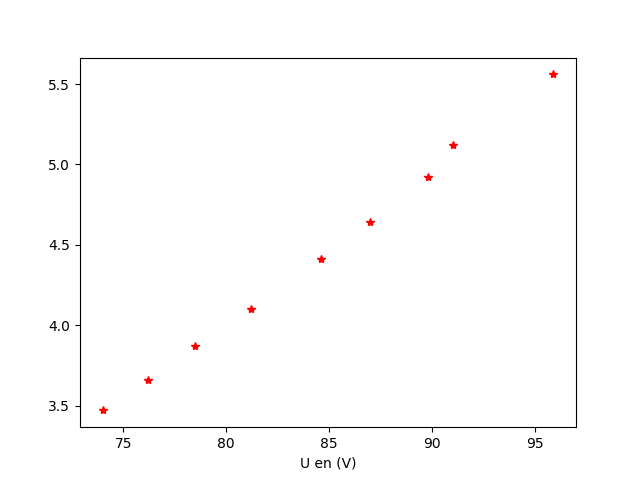
\includegraphics[width=0.5\textwidth]{tp06_durif_q02.png}
\end{center}